\documentclass[tikz,border=2pt]{standalone}
\usepackage{amsmath,amssymb}
\usepackage{pgfplots}
\pgfplotsset{compat=1.18}
\usetikzlibrary{arrows.meta}
\begin{document}
% u(w) = -e^{-w} (alpha = 1), loss X in {0,2} with probability 1/2 each: Pi = log((1+e^2)/2) ~ 1.43 solves
% E[u(Pi - X)] = u(0) = -1. The chord midpoint over Pi - E[X] ~ 0.43 sits at height -1, so by concavity Pi - E[X] >= 0.
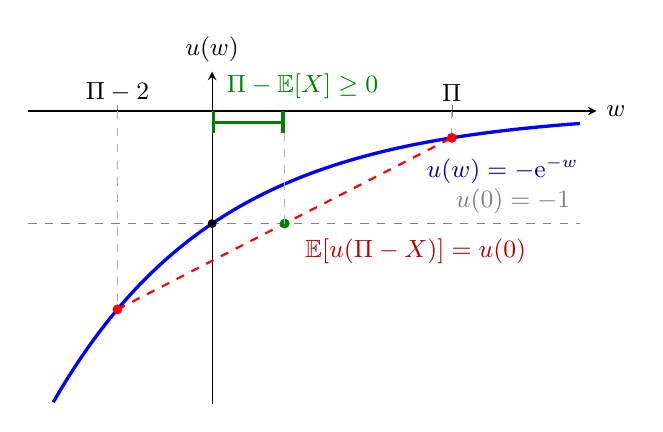
\begin{tikzpicture}[font=\small, >={Latex[length=2mm]}]
  \begin{axis}[
    axis lines=middle, xmin=-1.1, xmax=2.3, ymin=-2.6, ymax=0.35,
    xtick={-0.566,1.434}, xticklabels={$\Pi-2$,$\Pi$},
    ytick=\empty,
    xlabel={$w$}, ylabel={$u(w)$},
    xlabel style={anchor=west}, ylabel style={anchor=south},
    x tick label style={anchor=south, yshift=2pt},
    width=8.8cm, height=5.8cm, clip=false
    ]
    \addplot[blue, very thick, domain=-0.95:2.2, samples=80] {-exp(-x)};
    \node[blue!70!black, anchor=north east] at (axis cs:2.25,-0.32) {$u(w)=-\mathrm{e}^{-w}$};
    % reference level u(0)
    \draw[gray, thin, dashed] (axis cs:-1.1,-1) -- (axis cs:2.2,-1);
    \node[gray, anchor=south east] at (axis cs:2.2,-1) {$u(0)=-1$};
    % chord between the two net outcomes of the insurer
    \draw[red, thick, dashed] (axis cs:-0.566,-1.7616) -- (axis cs:1.434,-0.2384);
    \draw[gray!60, thin, dashed] (axis cs:-0.566,0) -- (axis cs:-0.566,-1.7616);
    \draw[gray!60, thin, dashed] (axis cs:1.434,0) -- (axis cs:1.434,-0.2384);
    \fill[red] (axis cs:-0.566,-1.7616) circle (1.8pt);
    \fill[red] (axis cs:1.434,-0.2384) circle (1.8pt);
    % expected utility equals u(0) at the mean net outcome
    \fill[green!50!black] (axis cs:0.434,-1) circle (1.8pt);
    \fill[black] (axis cs:0,-1) circle (1.6pt);
    \draw[gray!60, thin, dashed] (axis cs:0.434,-1) -- (axis cs:0.434,0);
    \draw[green!50!black, very thick, |-|] (axis cs:0,-0.1) -- (axis cs:0.434,-0.1);
    \node[green!50!black, anchor=south west] at (axis cs:0.03,0.02) {$\Pi-\mathbb{E}[X]\ge0$};
    \node[red!70!black, anchor=north west] at (axis cs:0.5,-1.05) {$\mathbb{E}[u(\Pi-X)]=u(0)$};
  \end{axis}
\end{tikzpicture}
\end{document}
